\documentclass[9pt,twocolumn,twoside,]{pnas-new}

%% Some pieces required from the pandoc template
\providecommand{\tightlist}{%
  \setlength{\itemsep}{0pt}\setlength{\parskip}{0pt}}

% Use the lineno option to display guide line numbers if required.
% Note that the use of elements such as single-column equations
% may affect the guide line number alignment.


\usepackage[T1]{fontenc}
\usepackage[utf8]{inputenc}



\templatetype{pnasresearcharticle}  % Choose template

\title{Ape cultures do not require behavior copying}

\author[a,1]{Alberto Acerbi}
\author[b]{William Daniel Snyder}
\author[b]{Claudio Tennie}

  \affil[a]{Centre for Culture and Evolution, Division of Psychology, Brunel
University London, Uxbridge, UB8 3PH, United Kingdom}
  \affil[b]{Faculty of Science, Department for Early Prehistory and Quaternary
Ecology, University of Tübingen, Schloß Hohentuebingen, Burgsteige 11,
72070, Tübingen, Germany}


% Please give the surname of the lead author for the running footer
\leadauthor{Acerbi}

% Please add here a significance statement to explain the relevance of your work
\significancestatement{Human culture is cumulative: it grows in complexity and efficiency,
drawing on the innovations of previous generations. In contrast, ape
cultures are not clearly cumulative. It has been proposed that human
cumulative culture depends on our ability to accurately transmit and
preserve information, and one basic mechanism for that is behavior
copying. At the same time, researchers have claimed that non-human apes
can also copy others' behavior. This raises a puzzling question: why are
ape cultures not cumulative? We show, through computer simulations, that
the patterns used to prove the existence of culture in wild ape
populations can be reproduced, in realistic conditions, without any
behavior copying. With this finding, the puzzle of why ape cultures are
not cumulative resolves itself.}


\authorcontributions{AA designed the research, developed the model and analysed the data, and
wrote the paper. WDS contributed the artwork for Figure 2 and gave
feedback on the paper. CT designed the research and wrote the paper.}



\correspondingauthor{\textsuperscript{} }

% Keywords are not mandatory, but authors are strongly encouraged to provide them. If provided, please include two to five keywords, separated by the pipe symbol, e.g:
 \keywords{  cultural transmission |  cultural evolution |  cumulative culture |  non-human great ape culture |  individual-based models |  behavior copying  } 

\begin{abstract}
We developed an individual-based model inspired by data on wild apes (1,
2) to test whether population-level distributions of traits suggestive
of cultures could emerge without behavior copying. We reproduce several
details of wild apes, including realistic demographic and spatial
features, and parametrised the range of genetic and ecological
variations between our populations. We also parametrised the degree to
which individual innovations are socially-mediated, i.e.~the degree to
which the probability for an individual to innovate a behavior is
dependent on the frequency of the same behavior in the population. Our
results show that, under realistic values of the main parameters, namely
null to medium importance of genetic variation, medium to high
importance of ecological variation, and various values of social
influence on innovations, we can reproduce distributions of behavioral
traits used to prove the existence of ape cultures. Our model reproduces
other features of the behaviors found in wild populations, including the
relative proportions of patterns of non-cultural behaviors (such as
behaviours present or absent in all sites, or behaviours absent because
of local ecological factors), as well as a correlation between
population size and the number of cultural traits in each site. Overall,
our results suggest that ape cultures can emerge without behavior
copying, providing an explanation as to why they do not appear to be
cumulative.
\end{abstract}

\dates{This manuscript was compiled on \today}
\doi{\url{www.pnas.org/cgi/doi/10.1073/pnas.XXXXXXXXXX}}

\begin{document}

% Optional adjustment to line up main text (after abstract) of first page with line numbers, when using both lineno and twocolumn options.
% You should only change this length when you've finalised the article contents.
\verticaladjustment{-2pt}

\maketitle
\thispagestyle{firststyle}
\ifthenelse{\boolean{shortarticle}}{\ifthenelse{\boolean{singlecolumn}}{\abscontentformatted}{\abscontent}}{}

% If your first paragraph (i.e. with the \dropcap) contains a list environment (quote, quotation, theorem, definition, enumerate, itemize...), the line after the list may have some extra indentation. If this is the case, add \parshape=0 to the end of the list environment.

\acknow{This project has received funding from the European Research Council
(ERC) under the European Union's Horizon 2020 research and innovation
programme (grant agreement n° 714658; STONECULT project). We would like
to than Mima Batalovic for the support provided, and Elisa Bandini, Alba
Motes Rodrigo, and Jonathan Reeves for comments on earlier versions of
the manuscript.}

Cumulative culture, the transmission and improvement of knowledge,
technologies, and beliefs from individual to individual, and from
generation to generation, is key to explain the extraordinary ecological
success of our species (3, 4). Which cognitive abilities underpin
human's cumulative cultural capacities, and how these abilities affect
the evolution of culture itself are among the most pressing questions of
evolutionary human science.

Many species are able to at least use social cues to adjust their
behavior. Various primates have been shown to posses traditions that are
socially influenced in this way (1, 2, 5). Humans, in contrast, have
cumulative culture. While there are various definitions of cumulative
culture (6), some of its characteristics are broadly accepted.
Cumulative culture requires the accumulation of cultural traits (more
cultural traits are present at generation \emph{g} than at time
\emph{g-1}), their improvement (cultural traits at generation \emph{g}
are more effective than at generation \emph{g-1}), and ratcheting (the
innovation of cultural traits at generation \emph{g} depends on the
presence of other traits at generation \emph{g-1}) (7).

While not all human culture needs to be supported by faithful copying
(8), cumulative culture depends on an ability to accurately transmit and
preserve new behaviors. Experiments have indeed shown that humans are
capable of copying behaviors, and that they routinely do so
cross-culturally (9, 10). More controversial is the claim that other
primate species copy behaviors. Arguments regarding the existence of
non-human great ape cultures based on behavior copying raise a puzzling
question: if other ape species can and do copy behaviors, why do they
not develop cumulative cultures? There are only two possible answers to
this question: either they do not copy behavior, or copying behavior
does not automatically lead to cumulative culture.

Primatologists have claimed the existence of ape cultures based on the
ability of behavior copying, drawing on observations conducted on wild
populations. For example, researchers examined the population-level
distribution of behaviors in populations of chimpanzees across seven
sites, and argued that the inter-site differences in the frequency of
behaviors proved the existence of behavior copying-based cultures in
these populations (1). We developed an individual-based model to assess
whether these patterns, and similar patterns in orangutans (2), actually
justify the conclusion that behavior copying is the underlying learning
mechanism. We reproduced several details of the original study (1),
including realistic demographic and spatial features, and effects of
ecological availability and genetic predisposition, to investigate
whether an equivalent distribution of behavioral traits could emerge in
the absence of any behavior copying. While our simulated ape species,
\emph{oranzees}, can be influenced by social cues (widespread in the
animal kingdom, and certainly present in all apes), we explicitly
excluded any behavior copying.

Our results show that, under realistic values of the main parameters, we
can reproduce the distribution of behavioral traits found in (1),
without any behavior copying required. In other words, as oranzees can
and do show cultural patterns resembling wild ape patterns, this shows
that such patterns do not constitute hard evidence that behavior copying
must have taken place.

\hypertarget{materials-and-methods}{%
\section*{Materials and methods}\label{materials-and-methods}}
\addcontentsline{toc}{section}{Materials and methods}

We built an individual-based model that reproduces a world inhabited by
six populations of ``oranzees'', a hypothetical ape species. The model
is spatially explicit: the oranzees populations are located at relative
positions analogous to the six chimpanzees sites in (1). This is
important to determine the potential genetic predispositions and
ecological availabilities associated with their possible behaviors (see
below). Population sizes are also taken from the sites in (1). Following
(11), we use data from (12), and we define population sizes as
\(N=\{20;42;49;76;50;95\}\).

Oranzees are subject to an age-dependent birth/death process, broadly
inspired by descriptions in (13). A time step \(t\) of the simulation
represents a month in oranzees' life. From when they are 25 years old
(\(t=300\)), there is a 1\% probability an oranzee will die each month,
or they die when they are 60 years old (\(t=720\)). The number of
individuals in the population is fixed, so each time an oranzee dies it
is replaced by a newborn.

A newborn oranzee does not yet show any behavior. Behaviors can be
innovated at each time step. The process of innovation is influenced by:
(i) the oranzees `state', which depends on the behaviors an individual
already possesses, (ii) the frequency of the behaviors already present
in the population (``socially-mediated reinnovation'' in (14)), and
(iii) the genetic propensity and ecological availability locally
associated with the behavior. At the beginning of the simulations, the
populations are randomly inizialised with individuals between 0 and 25
years old.

\hypertarget{format}{%
\subsection*{Oranzees' behaviors and state}\label{format}}
\addcontentsline{toc}{subsection}{Oranzees' behaviors and state}

In the oranzees' world, 64 behaviors are possible (targeting the 65
behaviors coded in (1), but making it an even number from modelling
convenience). Behaviors are divided into two categories: 32 social and
32 food-related behaviors. These figures where chosen to resemble the
behavioral categories considered in (1). Behaviors serve oranzees to
fulfill various goals. Oranzees have a `state' that is based on how many
goals are fulfilled in the two main categories of social and
food-related behaviors.

In the case of social behaviors, we assume four sub-categories (`play',
`display', `groom', `courtship'; note the names are only evocative),
each with eight possible different behaviors that serve the same goal. A
goal is considered fulfilled if an oranzee shows at least one behavior
out of the eight in the sub-category. Oranzees have a `state' that is
based on how many of the four goals are fulfilled. An oranzee has a
state value of \(0.25\) if, for example, it shows at least one behavior
in the category `play', and none of the others, and a state value of
\(1\) if it shows at least one behavior in each sub-category.
\(p_\text{social}\), the probability to innovate a social behavior, is
drawn from a normal distribution with mean equal to
\(1-state_\text{social}\).

Food-related behaviors are analogously divided into sub-categories.
Differently from social behaviors, there is a variable number of
behaviors in each sub-category. In addition, sub-categories are
associated to two different `nutrients', \emph{Y} and \emph{Z}. Here
individuals need to balance their nutritional intake, so that their
optimal diet consist in a roughly equal number of food for one and the
other nutrient. The state, for food-related behaviors, depends on the
total amount of food ingested \emph{and} on the balance between
nutrients. The state is calculated as the sum of each sub-category
fulfilled (as above, for this to happen there needs to be at least one
behavior present) minus the difference between the number of
sub-categories providing nutrient \emph{Y} and the number of
sub-categories providing nutrient \emph{Z}. We normalize the state
between \(0\) and \(1\), and, as above, \(p_\text{food}\) is then
calculated as \(1-state_\text{food}\).

\hypertarget{format}{%
\subsection*{Socially-mediated reinnovation}\label{format}}
\addcontentsline{toc}{subsection}{Socially-mediated reinnovation}

At each time step, all oranzees have a probability of innovation for
social and food-related behaviors calculated as described above. The
specific behavior an oranzee will innovate depends both on the frequency
of the behaviors already present in the population, and on the
ecological availability and genetic propensity associated to the
behavior. A further parameter of the model, \(S\), controls the
probability that each reinnovation is socially-mediated (14). When a
reinnovation is socially-mediated, the probability of innovating each
behavior \(B_i\) is weighted by its proportional instances in the
population among the behaviors of the same category (social or
food-related), so that common behaviors are more likely to be
reinnovated.

When the innovation is not socially-mediated, the probability of
innovating each behavior is random. Only one behavior per category can
be innovated at each time step.

\hypertarget{format}{%
\subsection*{Genetic propensity and ecological
availability}\label{format}}
\addcontentsline{toc}{subsection}{Genetic propensity and ecological
availability}

The behavior selected in the previous step is then innovated or not
according to its genetic propensity and, in case of food-related
behaviors, ecological availability.

Genetic propensity is a probability \(p_g(0,1)\), assigned independently
for each of the 64 behaviors. A parameter of the model, \(\alpha_g\),
determines the probability that the genetic propensity of each behavior
is equal for all the six populations or whether is different. If the
probability is equal, \(p_g\) is randomly drawn. If it is different, we
assign the propensity using a geographical gradient. We choose a random
point and calculate its distance to each population. Distances are then
transformed to \(p_g\) by rescaling them between 0 and 1, sso that for
the farthest site where \(p_g=0\), the associated behavior cannot
possibly be expressed (see SI). Notice that \(\alpha_g=0\) does not mean
that there are no genetic influences on the behavior, but that there are
no \emph{differences} between the populations with regard to this
aspect.

Ecological availability is a probability \(p_e(0,1)\) that represents
the likelihood of finding a resource, or its nutritional value, in each
site. Ecological availability is assigned only to food-related
behaviors, and it is calculated in the same way of \(p_g\), using the
parameter \(\alpha_e\) to determine the probability of ecological
availability being different in the six populations.

\begin{figure*}[h!]
\begin{center}
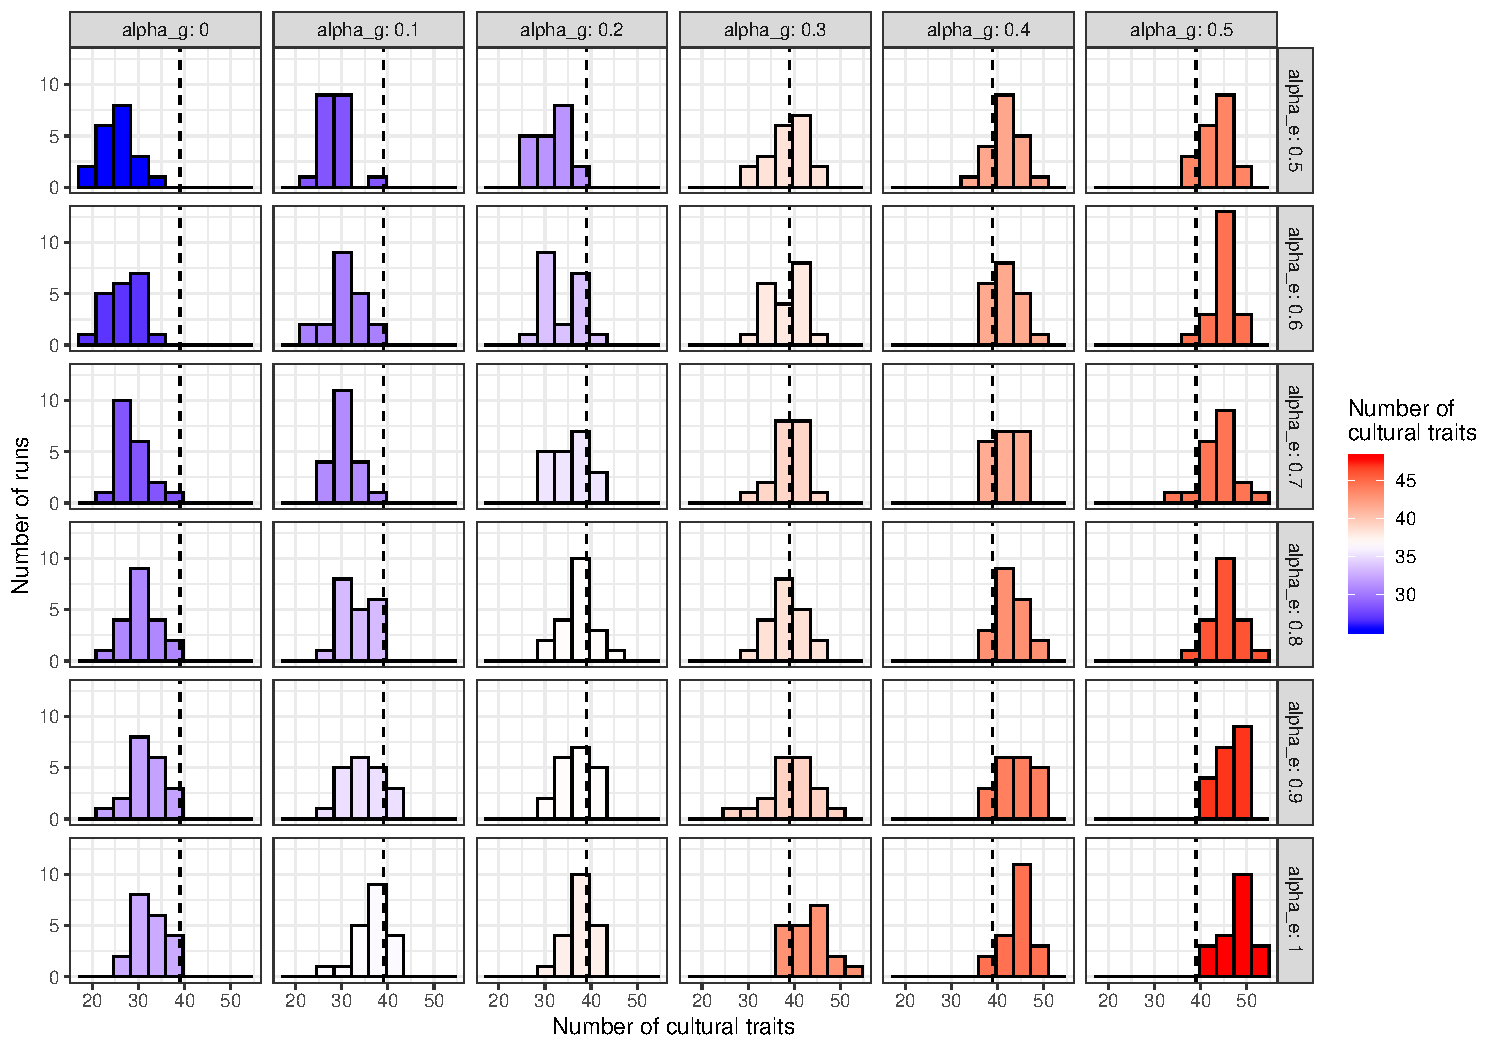
\includegraphics[width=10.8cm]{figures/figure_1.pdf}
\caption{Number of cultural traits in oranzees, when varying ecological and genetic diversity. Red colour indicates simulation runs that produced more than 38 cultural traits (the number of cultural traits identified in 1); blue colour indicates simulation runs that produced less than 38 cultural traits. For all simulations, $S=1$, $\alpha_e$ and $\alpha_g$ as indicated in the plot. $N=20$ runs for each parameters combination.}
\label{Figure1}
\end{center}
\end{figure*}

\hypertarget{format}{%
\subsection*{Model's output}\label{format}}
\addcontentsline{toc}{subsection}{Model's output}

We run simulations for \(t_\text{max}=6000\) (corresponding to 500 years
of oranzee-time). For each simulation, following (1), we classify each
behavior, in each population, as:

\begin{itemize}
\item
  \emph{customary}: a behavior observed in over 50\% of individuals in
  at least one age class (see SI for how age classes are defined in our
  model).
\item
  \emph{habitual}: a behavior observed in at least two individuals
  across the population.
\item
  \emph{present}: a behavior observed in at least one individual across
  the population.
\item
  \emph{absent}: a behavior not observed even once in the population.
\item
  \emph{ecological explanations}: a behavior that is absent due to a
  complete lack of local ecological availability (i.e., in our model,
  associated to \(p_e=0\)).
\end{itemize}

Notice that one additional category in (1) (\emph{unknown}, i.e. ``the
behavior has not been recorded, but this may be due to inadequacy of
relevant observational opportunities'') does not apply in our case,
because we have complete knowledge of the output of the simulations.

Finally, to test how well our model compares to wild apes, we calculate
the same ``patterns'' described in (1):

\begin{itemize}
\item
  \emph{A}: behavior absent at no site.
\item
  \emph{B}: behavior not achieving habitual frequencies at any site.
\item
  \emph{C}: behavior for which any absence can be explained by local
  ecological factors.
\item
  \emph{D}: behavior customary or habitual at some sites yet absent at
  others, with no ecological explanation, i.e.~behaviors defined as
  ``cultural''.
\end{itemize}

Further details of the model implementation and of how outputs are
processed are available in SI. The full code of the model allowing to
reproduce all our results, plus a detailed description of the model
development is available in a dedicated GitHub repository, at
\url{https://github.com/albertoacerbi/oranzees}.

\hypertarget{results}{%
\section*{Results}\label{results}}
\addcontentsline{toc}{section}{Results}

We are particularly interested in the realistic parameter conditions of
moderate to high environmental variability (i.e. \(\alpha_e\) from 0.5
to 1) and zero to moderate genetic differences (i.e. \(\alpha_g\) from 0
to 0.5). We ran 20 simulations for each combination (for a total of 600
runs). For all, reinnovation is socially-mediated (\(S=1\)). The results
show that various combinations of parameters produce a number of
cultural behaviors (pattern \emph{D}) consistent with the 38 found in
(1), in absence of any explicit copying mechanism being implemented (see
Figure \ref{Figure1}). In Figure \ref{Figure2}, we reproduce the output
of a run where 38 cultural behaviors were found, and how they were
classified in each of the six simulated populations, using a
visualization inspired by (1).

\begin{figure*}[h!]
\begin{center}
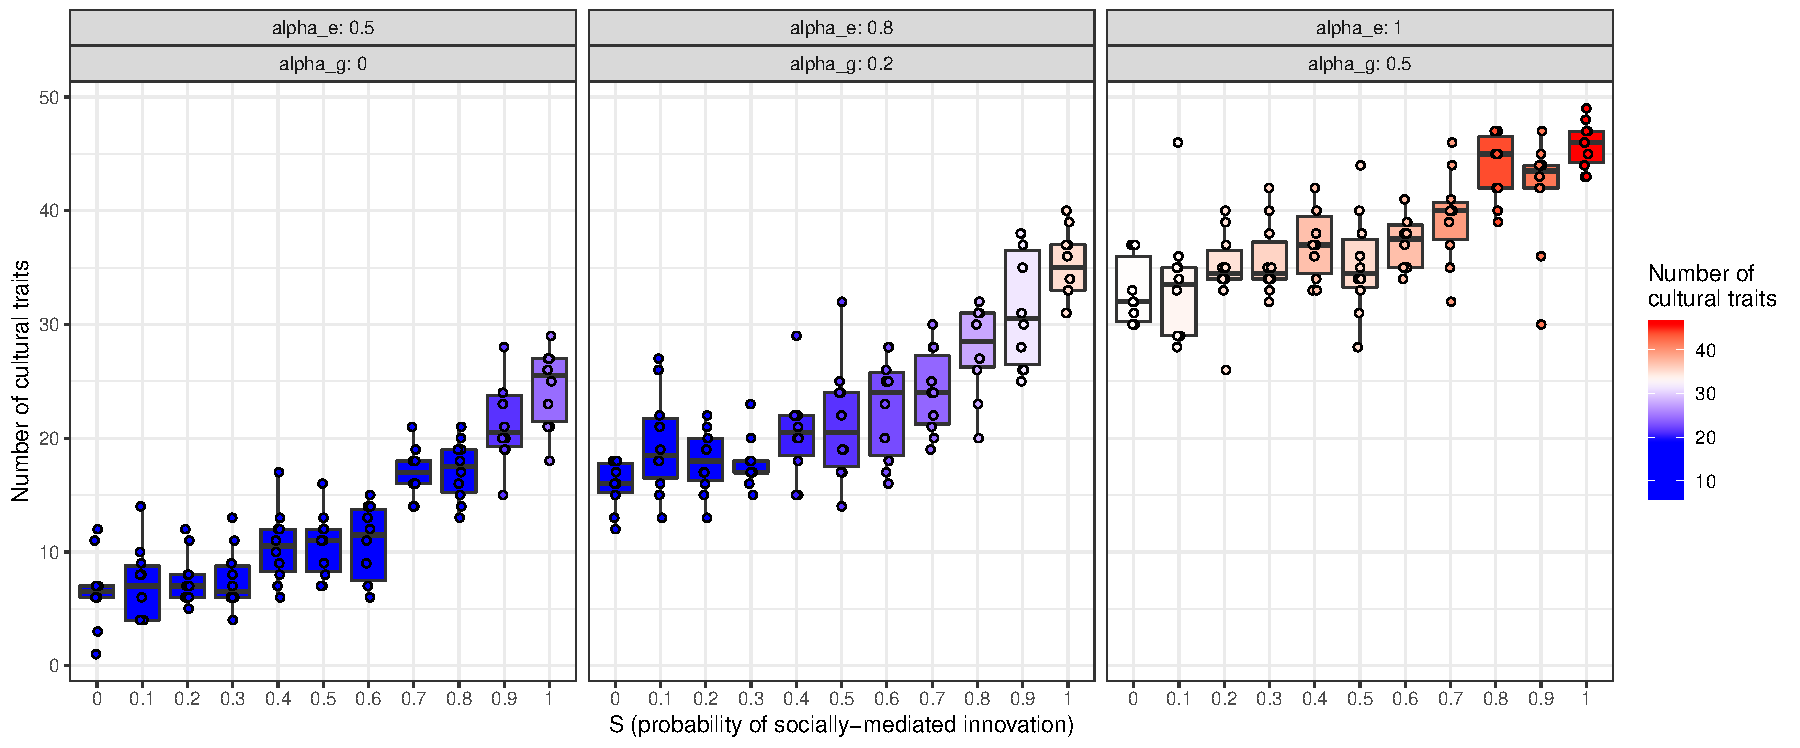
\includegraphics[width=13.8cm]{figures/figure_2.pdf}
\caption{Example of a simulation run that produces 38 cultural traits ($S=1$, $\alpha_e=0.8$, and $\alpha_g=0.2$). Color icons indicate customary behaviors; circular icons, habitual; monochrome icons, present; clear, absent;  horizontal bar, absent with ecological explanation. The names of the behaviors are only evocative, see SI for a complete list.}
\label{Figure2}
\end{center}
\end{figure*}

We also analysed the effect of the parameter \(S\) (proportion of
socially-mediated reinnovations), in three conditions (see Figure S4):
(a) no genetic differences and intermediate ecological differences
(compare to the high-left corner of Figure \ref{Figure1}, where with
\(S=1\) simulations produce less than 38 cultural behaviors), (b) one of
the conditions that produce good match with (1), namely \(\alpha_e=0.8\)
and \(\alpha_g=0.2\), and (c) intermediate genetic differences and high
ecological differences (compare to the low-right corner of Figure
\ref{Figure1}, where with \(S=1\) simulations produce more than 38
cultural behaviors). As expected, decreasing \emph{S} decreases the
number of cultural behaviors. Conditions where, with \(S=1\), there were
more than 38 cultural behaviors could still produce results analogous to
(1), given that not all reinnovations are socially mediated.

As a further proof of our model's fit with empiriclal data, our outputs
not only accurately reproduce the number of cultural behaviors (pattern
\emph{D}), but also the number of behaviors classified in the other
three patterns (\emph{A}, \emph{B}, \emph{C}, see above) in (1) (see
Figure S5).

Finally, we ran 100 simulations for one of the conditions where we have
a good match for the number of cultural behaviors in (1)
(\(\alpha_e=0.8;\alpha_g=0.2, S=1\)). In each simulation, we recorded,
for each population, the number of behaviors (habitual + customary +
present) that are also classified as cultural (see Figure S4). We find a
small, but significant, correlation between population size and number
of cultural traits (\(p<0.00001,\rho=0.2,N=600\)). In other words, our
model reproduces an effect of cultural accumulation (i.e.~increased
number of expressed behaviors) relative to population size possibly
found in real populations - see (11, 15, 16) - again, in absence of
behavior copying.

\hypertarget{discussion}{%
\section*{Discussion}\label{discussion}}
\addcontentsline{toc}{section}{Discussion}

We developed an individual-based model to examine under which conditions
a distribution of cultural traits analogous to the distribution reported
in (1) in chimpanzees could emerge, crucially, without allowing for the
existence of any behavior copying mechanism. We implemented several
details of the original wild ape study, including realistic demographic
and spatial features, as well as effects of genetic propensity and
ecological availability on the behaviors. Given the widespread
availability of non-copying variants of social learning across the
animal kingdom, we also included socially-mediated reinnovation, where
social learning merely catalyses individual reinnovation, without any
behavior copying (14).

Our main result is that we can reproduce the general pattern observed in
populations of wild apes under realistic values of the parameters of
genetic propensity and ecological availability, namely zero to medium
importance of genetic variation, and medium to high importance of
ecological variation. Our model cannot precisely determine which exact
values of these parameters produce the patterns in real populations of
chimpanzees (or other apes). However, we are confident that the range of
values explored, and the ease by which patterns of cultural behaviors
similar to (1) can be produced, strongly suggest that behavior copying
is not required for such patterns to emerge. Therefore, ape-like
cultural patterns (1, 2) do not and cannot pinpoint behavior copying
abilities. In addition, and as further support to our results, our model
not only reproduces the cultural behavioral patterns, but also the
proportions among the other patterns, i.e.~absent behaviors, behaviors
not achieving habitual frequencies at any site, and behaviors absent
because of ecological factors.

In our model, we focused on the mechanism of socially mediated
reinnovation, that is, we assumed that members of our hypothetical
species, oranzees, had a probability to reinnovate a specific behavior
stochastically linked to how many other oranzees in the population were
already showing this behavior. While this is a realistic assumption (17)
and while it reproduces in our model the chimpanzees' cultural pattern
observed in realistic conditions, our results demonstrate that it is not
necessary. Given certain combinations of parameters, such as higher
genetic and ecological diversities, the same population level pattern
can be obtained even when reinnovation is not socially mediated, i.e if
oranzees are not influenced by the behaviors of the other individuals in
their populations. That is, similar patterns can exist when the
underpinning individual-level mechanisms are not cultural even in a
minimal way (18).

Finally, our model reproduces a reported correlation between population
size and number of cultural traits in the six populations (11, 15, 16).
The magnitude of the effect is small, which is to be expected, given
that the presence of this correlation in real populations of (human and
non-human) apes is currently debated (19). Again, this correlation is
brought about without any behavior copying, so that there is no need to
invoke specific cultural reasons (e.g. (20)) to explain such pattern.

More generally, the results of our models suggest caution when deriving
individual-level mechanisms from population-level patterns (see also
(21, 22)). Cultural systems, as many others, exhibit equifinality: the
same global state can be produced by different local processes. Models
and experiments are crucial to test the plausibility of inferences going
from global to local properties.

In conclusion, our model strongly suggests that the data available on
the behavioral distributions of apes populations cannot demonstrate that
ape possess cultures influenced by behavior copying, let alone
\emph{requiring} behavior copying. This, in turn, may provide an
explanation to why ape cultures are not cumulative: as cumulative
culture requires at minimum behavior copying, we should not expect any
species lacking this mechanism to develop it.

\showmatmethods
\showacknow
\pnasbreak

\hypertarget{refs}{}
\leavevmode\hypertarget{ref-whiten_cultures_1999}{}%
1. Whiten A, et al. (1999) Cultures in chimpanzees. \emph{Nature}
399(6737):682--685.

\leavevmode\hypertarget{ref-van_schaik_orangutan_2003}{}%
2. van Schaik CP, et al. (2003) Orangutan Cultures and the Evolution of
Material Culture. \emph{Science} 299(5603):102--105.

\leavevmode\hypertarget{ref-henrich_secret_2015}{}%
3. Henrich J (2015) \emph{The Secret of Our Success: How Culture Is
Driving Human Evolution, Domesticating Our Species, and Making Us
Smarter} (Princeton University Press, Princeton \& Oxford).

\leavevmode\hypertarget{ref-boyd_different_2017}{}%
4. Boyd R (2017) \emph{A Different Kind of Animal: How Culture
Transformed Our Species} (Princeton University Press, Princeton).

\leavevmode\hypertarget{ref-whiten_primate_2000}{}%
5. Whiten A (2000) Primate culture and social learning. \emph{Cognitive
Science} 24(3):477--508.

\leavevmode\hypertarget{ref-mesoudi_what_2018}{}%
6. Mesoudi A, Thornton A (2018) What is cumulative cultural evolution?
\emph{Proceedings of the Royal Society B: Biological Sciences}
285(1880):20180712.

\leavevmode\hypertarget{ref-acerbi_cultural_2019}{}%
7. Acerbi A (2019) \emph{Cultural Evolution in the Digital Age} (Oxford
University Press, Oxford, New York).

\leavevmode\hypertarget{ref-morin_how_2015}{}%
8. Morin O (2015) \emph{How Traditions Live and Die} (Oxford University
Press, London \& New York).

\leavevmode\hypertarget{ref-nielsen_overimitation_2010}{}%
9. Nielsen M, Tomaselli K (2010) Overimitation in Kalahari Bushman
Children and the Origins of Human Cultural Cognition:
\emph{Psychological Science}.
doi:\href{https://doi.org/10.1177/0956797610368808}{10.1177/0956797610368808}.

\leavevmode\hypertarget{ref-berl_cultural_2015}{}%
10. Berl REW, Hewlett BS (2015) Cultural Variation in the Use of
Overimitation by the Aka and Ngandu of the Congo Basin. \emph{PLOS ONE}
10(3):e0120180.

\leavevmode\hypertarget{ref-lind_number_2010}{}%
11. Lind J, Lindenfors P (2010) The Number of Cultural Traits Is
Correlated with Female Group Size but Not with Male Group Size in
Chimpanzee Communities. \emph{PLoS ONE} 5(3).
doi:\href{https://doi.org/10.1371/journal.pone.0009241}{10.1371/journal.pone.0009241}.

\leavevmode\hypertarget{ref-wrangham_why_2000}{}%
12. Wrangham RW (2000) Why are male chimpanzees more gregarious than
mothers? A scramble competition hypothesis. \emph{Primate Males: Causes
and Consequences of Variation in Group Composition} (Cambridge
University Press, Cambridge), pp 248--258.

\leavevmode\hypertarget{ref-hill_mortality_2001}{}%
13. Hill K, et al. (2001) Mortality rates among wild chimpanzees.
\emph{Journal of Human Evolution} 40(5):437--450.

\leavevmode\hypertarget{ref-bandini_spontaneous_2017}{}%
14. Bandini E, Tennie C (2017) Spontaneous reoccurrence of ``scooping'',
a wild tool-use behaviour, in naïve chimpanzees. \emph{PeerJ} 5:e3814.

\leavevmode\hypertarget{ref-whiten_evolution_2007}{}%
15. Whiten A, Schaik CP van (2007) The evolution of animal ``cultures''
and social intelligence. \emph{Philosophical Transactions of the Royal
Society B: Biological Sciences} 362(1480):603--620.

\leavevmode\hypertarget{ref-kuhl_human_2019}{}%
16. Kühl HS, et al. (2019) Human impact erodes chimpanzee behavioral
diversity. \emph{Science} 363(6434):1453--1455.

\leavevmode\hypertarget{ref-tennie_evidence_2010}{}%
17. Tennie C, Call J, Tomasello M (2010) Evidence for Emulation in
Chimpanzees in Social Settings Using the Floating Peanut Task.
\emph{PLoS ONE} 5(5).
doi:\href{https://doi.org/10.1371/journal.pone.0010544}{10.1371/journal.pone.0010544}.

\leavevmode\hypertarget{ref-neadle_food_2017}{}%
18. Neadle D, Allritz M, Tennie C (2017) Food cleaning in gorillas:
Social learning is a possibility but not a necessity. \emph{PLOS ONE}
12(12):e0188866.

\leavevmode\hypertarget{ref-vaesen_population_2016}{}%
19. Vaesen K, Collard M, Cosgrove R, Roebroeks W (2016) Population size
does not explain past changes in cultural complexity. \emph{Proceedings
of the National Academy of Sciences of the United States of America}
113(16):E2241--2247.

\leavevmode\hypertarget{ref-henrich_demography_2004}{}%
20. Henrich J (2004) Demography and Cultural Evolution: How Adaptive
Cultural Processes can Produce Maladaptive Losses: The Tasmanian Case.
\emph{American Antiquity} 69(2):197--214.

\leavevmode\hypertarget{ref-acerbi_conformity_2016}{}%
21. Acerbi A, Van Leeuwen EJ, Haun DB, Tennie C (2016) Conformity cannot
be identified based on population-level signatures. \emph{Scientific
reports} 6:36068.

\leavevmode\hypertarget{ref-barrett_equifinality_2019}{}%
22. Barrett BJ (2019) Equifinality in empirical studies of cultural
transmission. \emph{Behavioural Processes} 161:129--138.



% Bibliography
% \bibliography{pnas-sample}

\end{document}

